% Architecture diagram for HDM paper
% Compile with: pdflatex architecture_diagram.tex

\documentclass[border=5pt]{standalone}
\usepackage{tikz}
\usetikzlibrary{shapes.geometric, arrows.meta, positioning, fit, backgrounds, calc}

\definecolor{upperlayer}{RGB}{230, 190, 230}
\definecolor{lowerlayer}{RGB}{190, 220, 255}
\definecolor{guidance}{RGB}{255, 230, 180}
\definecolor{scoring}{RGB}{180, 255, 200}
\definecolor{emergency}{RGB}{255, 200, 200}

\begin{document}

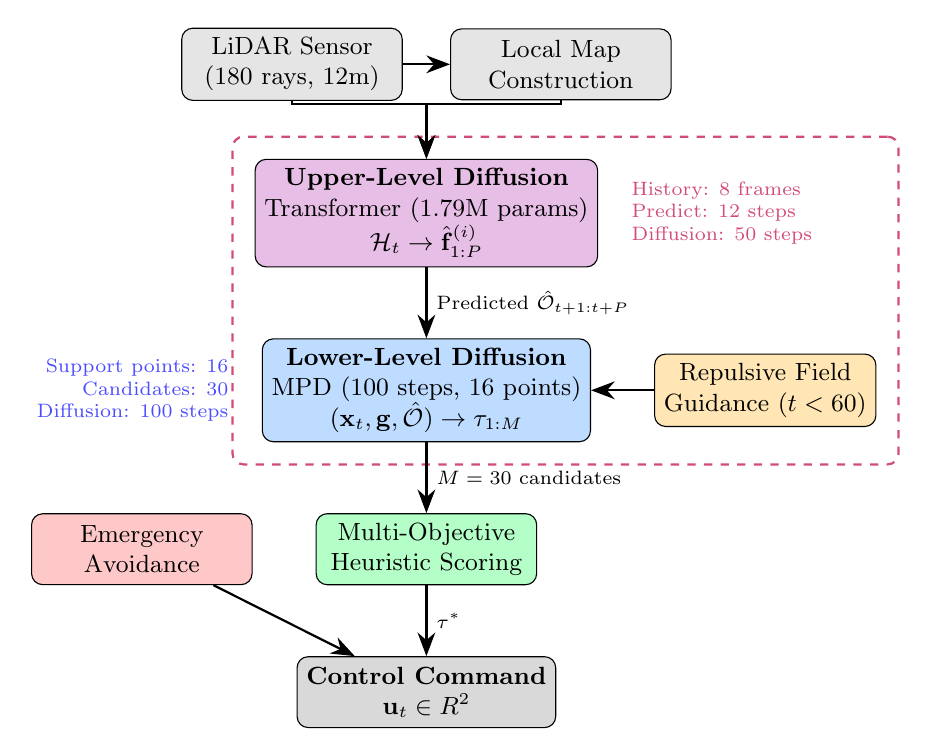
\begin{tikzpicture}[
    node distance=0.8cm,
    box/.style={rectangle, rounded corners, draw, minimum width=2.8cm, minimum height=0.9cm, align=center, font=\small},
    arrow/.style={-{Stealth[length=3mm]}, thick},
    label/.style={font=\footnotesize\bfseries, align=center}
]

% Input layer
\node[box, fill=gray!20] (lidar) {LiDAR Sensor\\(180 rays, 12m)};
\node[box, fill=gray!20, right=0.6cm of lidar] (localmap) {Local Map\\Construction};

% Upper-level diffusion
\node[box, fill=upperlayer, below=1.2cm of $(lidar)!0.5!(localmap)$] (upper) {
    \textbf{Upper-Level Diffusion}\\
    Transformer (1.79M params)\\
    $\mathcal{H}_t \rightarrow \hat{\mathbf{f}}_{1:P}^{(i)}$
};

% Lower-level diffusion
\node[box, fill=lowerlayer, below=0.9cm of upper, minimum height=1.1cm] (lower) {
    \textbf{Lower-Level Diffusion}\\
    MPD (100 steps, 16 points)\\
    $(\mathbf{x}_t, \mathbf{g}, \hat{\mathcal{O}}) \rightarrow \boldsymbol{\tau}_{1:M}$
};

% Repulsive guidance
\node[box, fill=guidance, right=0.8cm of lower] (guidance) {
    Repulsive Field\\
    Guidance ($t<60$)
};

% Trajectory scoring
\node[box, fill=scoring, below=0.9cm of lower] (scoring) {
    Multi-Objective\\
    Heuristic Scoring
};

% Emergency avoidance
\node[box, fill=emergency, left=0.8cm of scoring] (emergency) {
    Emergency\\
    Avoidance
};

% Output
\node[box, fill=gray!30, below=0.9cm of scoring] (output) {
    \textbf{Control Command}\\
    $\mathbf{u}_t \in \mathbb{R}^2$
};

% Arrows
\draw[arrow] (lidar) -- (localmap);
\draw[arrow] (localmap) -- ++(0, -0.5) -| (upper);
\draw[arrow] (lidar) -- ++(0, -0.5) -| (upper);
\draw[arrow] (upper) -- node[right, font=\scriptsize] {Predicted $\hat{\mathcal{O}}_{t+1:t+P}$} (lower);
\draw[arrow] (guidance) -- (lower);
\draw[arrow] (lower) -- node[right, font=\scriptsize] {$M=30$ candidates} (scoring);
\draw[arrow] (emergency) -- (output);
\draw[arrow] (scoring) -- node[right, font=\scriptsize] {$\boldsymbol{\tau}^*$} (output);

% Background boxes
\begin{scope}[on background layer]
    \node[draw=purple!70, thick, dashed, rounded corners, fit=(upper)(lower)(guidance), inner sep=8pt, label={[font=\footnotesize\bfseries]above:Hierarchical Diffusion Model}] {};
\end{scope}

% Annotations
\node[right=0.3cm of upper, font=\scriptsize, align=left, text=purple!70] {
    History: 8 frames\\
    Predict: 12 steps\\
    Diffusion: 50 steps
};

\node[left=0.3cm of lower, font=\scriptsize, align=right, text=blue!70] {
    Support points: 16\\
    Candidates: 30\\
    Diffusion: 100 steps
};

\end{tikzpicture}

\end{document}
